%************************************************
\chapter{Understanding Genetics Using Drosophila Melanogaster}\label{exp2}
%************************************************
\section{Objective}
To understand how the genes for eye colour are inherited in Drosophila, by setting up various crosses of the pure breeds which have only.

\section{Material Required}
	\begin{enumerate}
		\item Virgin Drosophila (Wild type, Scarlet and Red eyed)
		\item Wild type
		\item Scarlet
		\item White
		\item Vials containing food
		\item Empty Vials
		\item Cotton plugs
		\item Ice box and Ice pack
		\item Paint Brush
		\item Binocular Microscope
		\item Needles
		\item Tissue Paper
		\item Yeast as extra food
		\item Ether as anaesthesia
		\item Funnel
	\end{enumerate}

\section{Idea}
	The wild type (the ``normal'') of drosophila has Red eye colour. We also have a bunch of mutants. In this experiment we'll use White and Scarlet eye coloured mutants. We take their pure breeds and do the crosses as listed in \autoref{2_f1_crosses}. For the actual experiment, we use 2 females and 2 males for each type. Also, we do the same cross thrice to be moderately rigorous.
	\marginpar{\Lisa Pure Breed: When bread amongst themselves, they yield the same phenotype}

	\begin{table}
		\myfloatalign
		\begin{tabularx}{\textwidth}{Xll}
			\hline%
			Red (wild type) Male & White Female\\
			Red (wild type) Female & White Male\\
			Red (wild type) Male & Scarlet Female\\
			Red (wild type) Female & Scarlet Male\\
			\hline%
		\end{tabularx}
		\caption{F1 Crosses}
		\label{2_f1_crosses}
	\end{table}

	We then observe their phenotype (eye colour) in the generation obtained, lets call them F1. We then note that in F1, for a given sex, there's only one phenotype. We count them. Then we self them and again observe their phenotype. (although this time its more painful, since we've to observe males females and their phenotypes, so no running away from the microscope for amatures like us!) 
	\par 
	The objective is to investigate the mechanism by which genes are passed from one generation to another and since this experiment got Morgen the Nobel, therefore its rather obvious that there's more to it than the typical mono-hybrid cross.

\section{Procedure Essentials}
	There is not much significance of re-writing the detailed sequential procedure. The repetitive modules, interesting, unexpected steps have been listed here.
	\begin{enumerate}
		\item When labels were put on the vials that were intended to kept in the freezer, they were taped. Sounds trivial but was very essential.
		\item The method of setting up a cross:
			\begin{enumerate}
				\item Took the vials, dried them and cooled them using ice. \marginpar{\Lisa We dry them cause else the moisture condenses and that's not good for the flies}
				\item Then transferred the flies into these vials, put the cotton plug swiftly and put it back for cooling (for retaining the low temperature)
				\item When the flies become inactive, put them on an icepack with a tissue paper on top, which doesn't have air bubbles. \marginpar{\Lisa The air bubbles will be at a higher temperature!}
				\item Then selected the required males and females with the desired phenotypes, by observing them under a microscope if the need be, and transferred them into a new food vial, and plugged the cotton.
				\item Kept the food vial horizontal until the flies start moving and then restored the vials to a vertical position. \marginpar{\Lisa To prevent the unconscious flies from getting stuck on the vials}
				\item Labelled the vial accordingly and stored it at 25$^{0}$C, in an incubator and waited for about 36 hours.
				\item Checked if there were enough flies. If not, waited for another 12 hours. Then the parent flies were discarded in a soap solution. \marginpar{\Lisa To prevent overcrowding of eggs.}
				\item Periodically, the new flies were transferred into new vials. \marginpar{\Bart How does overcrowding make a difference here}
			\end{enumerate}
		\item We used an improvised method for keeping the flies anaesthetized as listed below:
			\begin{enumerate}
				\item Took a petridish and filled it with crushed ice to the brim, without closing the lid.
				\item Using an aluminium foil, covered the surface of the petridish.
				\item Put a tissue paper on it
			\end{enumerate}
	\end{enumerate}

\section{Observations and Analysis}
	Observations in this experiment are restricted to the number of flies of specific eye colour and sex, in a given generation. As described earlier, F1 is the first generation and F2 is the second generation. For various crosses, the observations have been summarized as below:
	\begin{enumerate}
		\item Cross 1: Scarlet Male with Red Female
			\begin{enumerate}
				\item F1: \autoref{2_Af1}
				\item F2: \autoref{2_Af2}
			\end{enumerate}
		\item Cross 2: Scarlet Male with Red Female
			\begin{enumerate}
				\item F1: \autoref{2_Bf1}
				\item F2: \autoref{2_Bf2}
			\end{enumerate}
		\item Cross 3: White Male with Red Female
			\begin{enumerate}
				\item F1: \autoref{2_Cf1}
				\item F2: \autoref{2_Cf2} \footnote{total's excluding Vial 1}
			\end{enumerate}
		\item Cross 4: Red Male with White Female
			\begin{enumerate}
				\item F1: \autoref{2_Df1}
				\item F2: \autoref{2_Df2}
			\end{enumerate}
	\end{enumerate}
	For analysing the data, we used what's known as a $\chi^{2}$ test. The mathematical analysis has been appended, in accordance to which, our experiment confirmed the expected hypothesis\footnote{However, we did reject data collected from one vial in Cross 3, as it had been contaminated}. For Cross 1 and 2, with parents as Scarlet and Red, the hypothesis that Scarlet Eye colour is a typical single locus, recessive trait was verified. Quantitatively, Cross 1 was found to have $\chi^{2}=0.0$, which was rather co-incidental \marginpar{\Homer Don't think we performed the experiment really well!}, and for Cross 2, $\chi^{2}$ was found to be $0.31$ which is less than 3.148, the value corresponding to $5\%$ and single degree of freedom.\\
	Now for the more interesting ones, Cross 3 and Cross 4, were subjected to two tests. First we assumed a null hypothesis similar to that of the first case, viz. White Eye colour is a typical single locus, recessive trait. For this, Cross 3 yielded $\chi^{2}>12.9$. Cross 4 produced results distinctly in contrast with the null hypothesis: 
		\begin{enumerate}
			\item A significant number of White Female flies were observed which according to the hypothesis should \emph{not} be observed at all
			\item \emph{No} Red Females were observed, which according to the hypothesis should constitute \emph{half} the progeny.
		\end{enumerate}
	This confirmed that the inheritance of White Eye colour can't be explained by the hypothesis.
	\par
	The other null hypothesis was that the White Eye colour trait is recessive and sits on the X chromosome. According to this hypothesis, $\chi^{2}$ was found to be $0.601$ and $1.91$ for Cross 3 and 4 respectively. Since both these numbers were found to be less than 3.841, the value corresponding to, again $5\%$ and single degree of freedom, \marginpar{\Lisa Degree of freedom in this case was $(n-1)(n-1)=1$, for $n=2$} the null hypothesis satisfactorily explains inheritance of the White Eye colour.
	\begin{table}
		\myfloatalign
		\begin{tabularx}{\textwidth}{Xlll}
			\hline%
			F1 & \tableheadline{Red Male} & \tableheadline{Red Female} \\			
			\tableheadline{Vial 1} & 57  & 63 \\
			\tableheadline{Vial 2} & 32 & 27\\
			\tableheadline{Vial 3} & 28 & 40\\
			\hline%
			\tableheadline{Total} & 117 & 130\\
		\end{tabularx}
		\caption{Cross 1: F1 Crosses (Scarlet Male with Red Female)}
		\label{2_Af1}
	\end{table}
	

	\begin{table}
		\myfloatalign
		\begin{tabularx}{\textwidth}{Xllll}
			\hline%
			F2 & \tableheadline{Red Male} & \tableheadline{Red Female} & \tableheadline{Scarlet Male} & \tableheadline{Scarlet Female}\\			
			\tableheadline{Vial 1} & 41 & 55 & 18 & 12\\
			\tableheadline{Vial 2} & 45 & 58 & 21 & 14\\
			\tableheadline{Vial 3} & 42 & 59 &  9 & 26\\
			\hline%
			\tableheadline{Total} & Red & 300 & Scarlet & 100\\
		\end{tabularx}

		\caption{Cross 1: F2 Crosses (Red (F1) Male with Red (F1) Female)}
		\label{2_Af2}
	\end{table}


	\begin{table}
		\myfloatalign
		\begin{tabularx}{\textwidth}{Xlll}
			\hline%
			F1 & \tableheadline{Red Male} & \tableheadline{Red Female} \\			
			\tableheadline{Vial 1} & 47 & 47\\
			\tableheadline{Vial 2} & 45 & 56 \\
			\tableheadline{Vial 3} & 68 & 73 \\
			\hline%
			\tableheadline{Total} & 160 & 176\\
		\end{tabularx}
		\caption{Cross 2: F1 Crosses (Red Male with Scarlet Female)}
		\label{2_Bf1}
	\end{table}
	

	\begin{table}
		\myfloatalign
		\begin{tabularx}{\textwidth}{Xllll}
			\hline%
			F2 & \tableheadline{Red Male} & \tableheadline{Red Female} & \tableheadline{Scarlet Male} & \tableheadline{Scarlet Female}\\			
			\tableheadline{Vial 1} & 23 & 50 & 13 & 14\\
			\tableheadline{Vial 2} & 42 & 36 & 19 & 13\\
			\tableheadline{Vial 3} & 24 & 27 &  5 & 9\\
			\hline%
			\tableheadline{Total} & Red & 202 & Scarlet & 73\\
		\end{tabularx}

		\caption{Cross 2: F2 Crosses (Red (F1) Male with Red (F1) Female)}
		\label{2_Bf2}
	\end{table}


	\begin{table}
		\myfloatalign
		\begin{tabularx}{\textwidth}{Xlll}
			\hline%
			F1 & \tableheadline{Red Male} & \tableheadline{Red Female} \\			
			\tableheadline{Vial 1} & 96  & 74 \\
			\tableheadline{Vial 2} & 76 & 102\\
			\tableheadline{Vial 3} & 98 & 72\\
			\hline%
			\tableheadline{Total} & 117 & 130\\
		\end{tabularx}
		\caption{C: F1 Crosses (White Male with Red Female)}
		\label{2_Cf1}
	\end{table}
	

	\begin{table}
		\myfloatalign
		\begin{tabularx}{\textwidth}{Xllll}
			\hline%
			F2 & \tableheadline{White Male} & \tableheadline{White Female} & \tableheadline{Red Male} & \tableheadline{Red Female}\\			
			\tableheadline{Vial 1} & 11 & 16 & 7  & 16\\
			\tableheadline{Vial 2} & 28 & 60 & 18 & 0\\
			\tableheadline{Vial 3} & 11 & 34 & 22 & 0\\
			\hline%
			\tableheadline{Total} & 39 & 94 & 40 & 0\\
		\end{tabularx}

		\caption{C: F2 Crosses (Red (F1) Male with Red (F1) Female)}
		\label{2_Cf2}
	\end{table}

	\begin{table}
		\myfloatalign
		\begin{tabularx}{\textwidth}{Xlll}
			\hline%
			F1 & \tableheadline{White Male} & \tableheadline{Red Female} \\			
			\tableheadline{Vial 1} & 85 & 70 \\
			\tableheadline{Vial 2} & 62 & 68\\
			\tableheadline{Vial 3} & 54 & 75\\
			\hline%
			\tableheadline{Total} & 201 & 213\\
		\end{tabularx}
		\caption{Cross 4: F1 Crosses (Red Male with White Female)}
		\label{2_Df1}
	\end{table}
	

	\begin{table}
		\myfloatalign
		\begin{tabularx}{\textwidth}{Xllll}
			\hline%
			F2 & \tableheadline{Red Male} & \tableheadline{Red Female} & \tableheadline{White Male} & \tableheadline{White Female}\\			
			\tableheadline{Vial 1} & 15 & 22 & 11 & 21\\
			\tableheadline{Vial 2} & 17 & 14 & 12 & 12\\
			\tableheadline{Vial 3} & 24 & 34 & 39 & 37\\
			\hline%
			\tableheadline{Total} & Red & 300 & White & 100\\
		\end{tabularx}

		\caption{Cross 4: F2 Crosses (Red (F1) Male with Red (F1) Female)}
		\label{2_Df2}
	\end{table}

	%\Venus \Mars
	% \male \mars
\section{Discussion}
	So far so good, but here's the catch; if there's a locus for eye colour on the autosome, \emph{and} there's a locus for eye colour on the X chromosome, what happens when you attempt to cross a Scarlet with a White?
	\par
	We could perform a experiments and find out. Others who've already performed and analysed them, explain the phenomenon as the following: the eye colour, is controlled by a two pathways. When both pathways are functional, the wild type, Red eye colour is obtained. When both are non-functional, then White eye colour is obtained. The other two cases result in Brown and Scarlet, as is given in \autoref{2_eyecolour}.

	\begin{figure}[bth]
		\begin{center}
			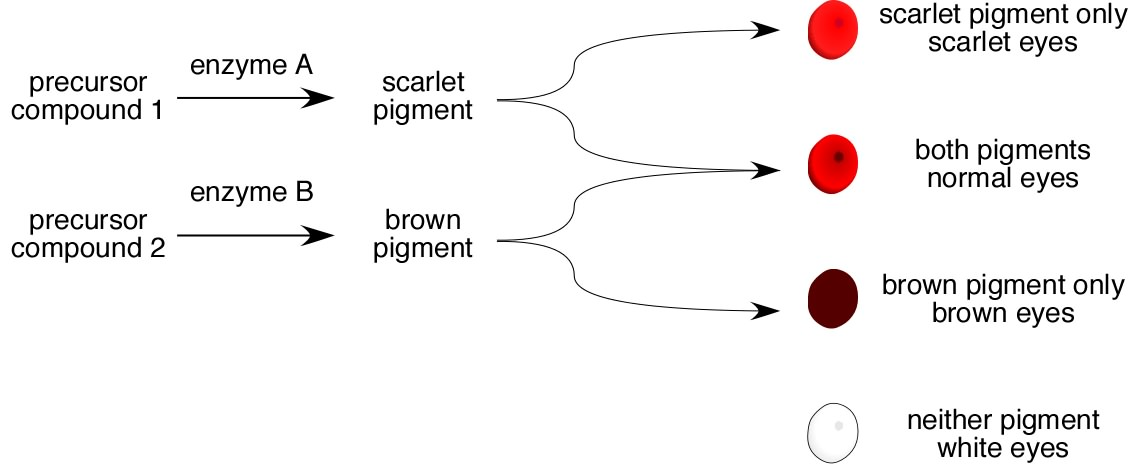
\includegraphics[width=1.0\linewidth]{gfx/eyecolor}
		\end{center}
	\caption[Drosophila eye colour]{Drosophila eye colour}
	\label{2_eyecolour}
	\end{figure}

\section{Reference}
	\url{http://www.indiana.edu/~oso/lessons/Genetics/bw_st.html}

\section{Acknowledgement}
	I would like to sincerely thank Mr. Biplob Nandy, who helped us perform the experiment as a team member. I also acknowledge Vivek Sagar for his contribution to the project, as a team member. I thank our instructor, Dr. N. G. Prasad for his expert guidance and novel teaching methods.